\documentclass[11pt,letterpaper]{article}

%%%%%%%%%%%%%%%%%%%%%%%%%%%%%%%%%%%
% IMPORTACIÓN DE CONFIGURACIONES
%%%%%%%%%%%%%%%%%%%%%%%%%%%%%%%%%%%

\input{configuracion}

%%%%%%%%%%%%%%%%%%%%%%%%%%%%
% INICIO DE DOCUMENTO
%%%%%%%%%%%%%%%%%%%%%%%%%%%%

\begin{document}

%%%%%%%%%%%%%%%%%%%%%%%%%%%%
% ENCABEZADO
%%%%%%%%%%%%%%%%%%%%%%%%%%%%
\begin{center}
    \begin{minipage}{3cm}
    	\begin{center}
    		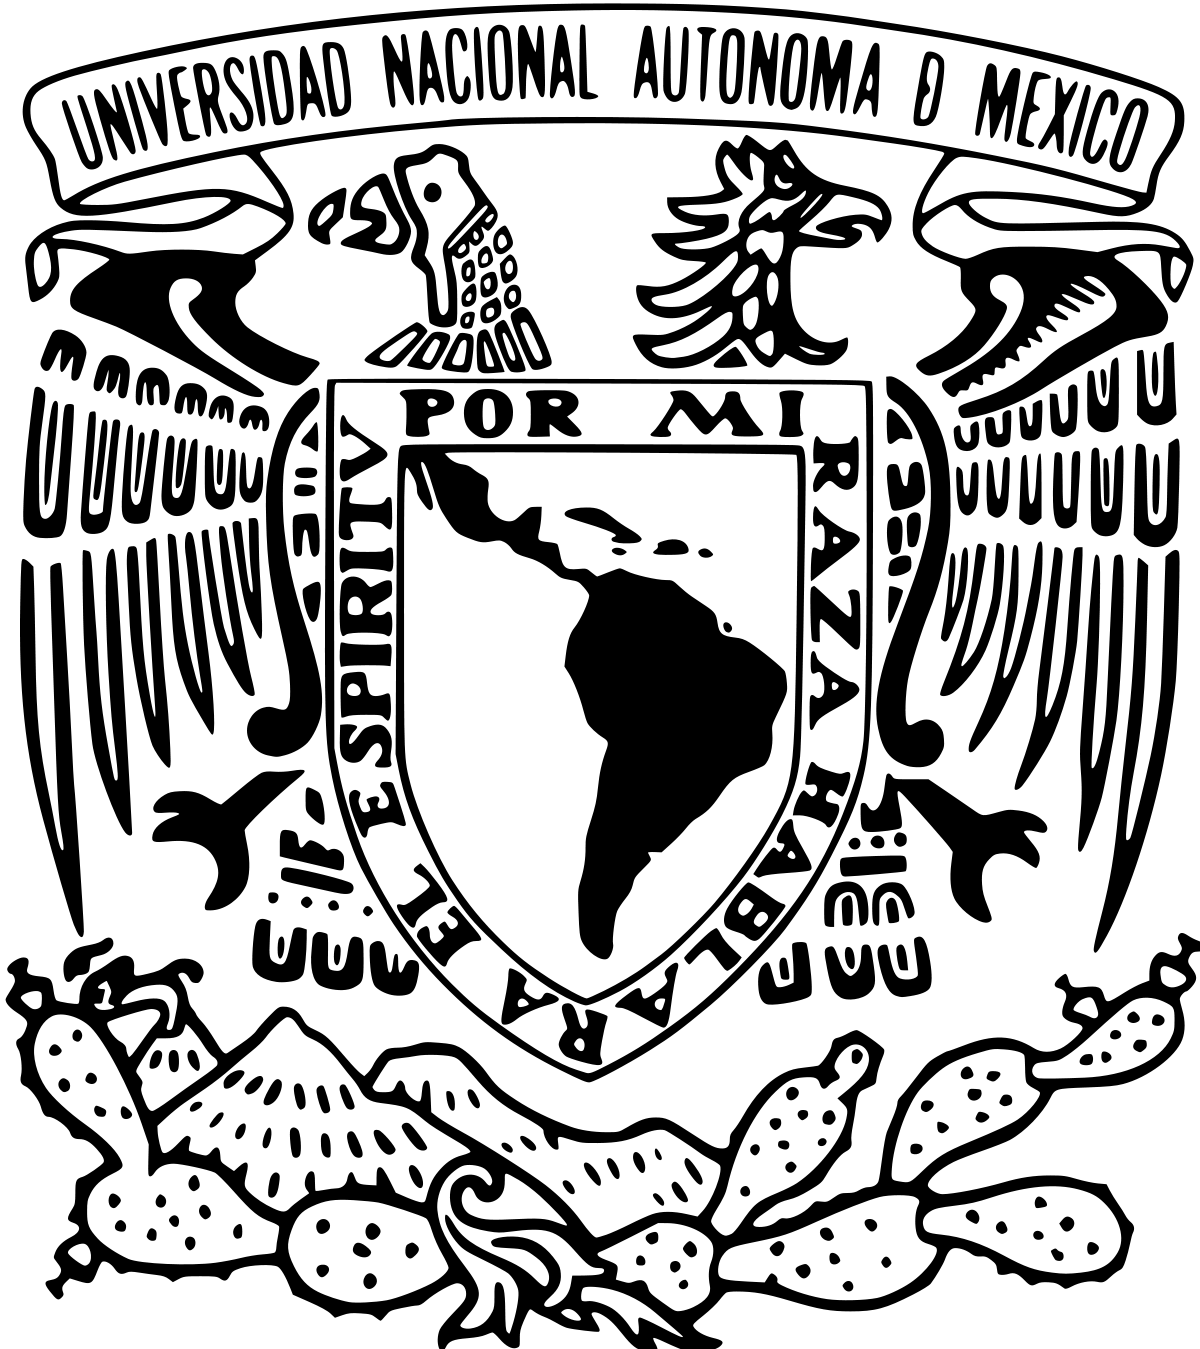
\includegraphics[height=3.4cm]{Logo_UNAM.png}
    	\end{center}
    \end{minipage}\hfill
    \begin{minipage}{10cm}
    	\begin{center}
    	\textbf{\large Universidad Nacional Autónoma de México}\\[0.1cm]
        \textbf{Facultad de Ciencias}\\[0.1cm]
        \textbf{Geometría Analítica II $|$ Grupo 4092}\\[0.1cm]
        Quizz 2\\[0.1cm]
        Martínez Castro Alvaro Leonardo\\[0.1cm]
        \today
    	\end{center}
    \end{minipage}\hfill
    \begin{minipage}{3cm}
    	\begin{center}
    		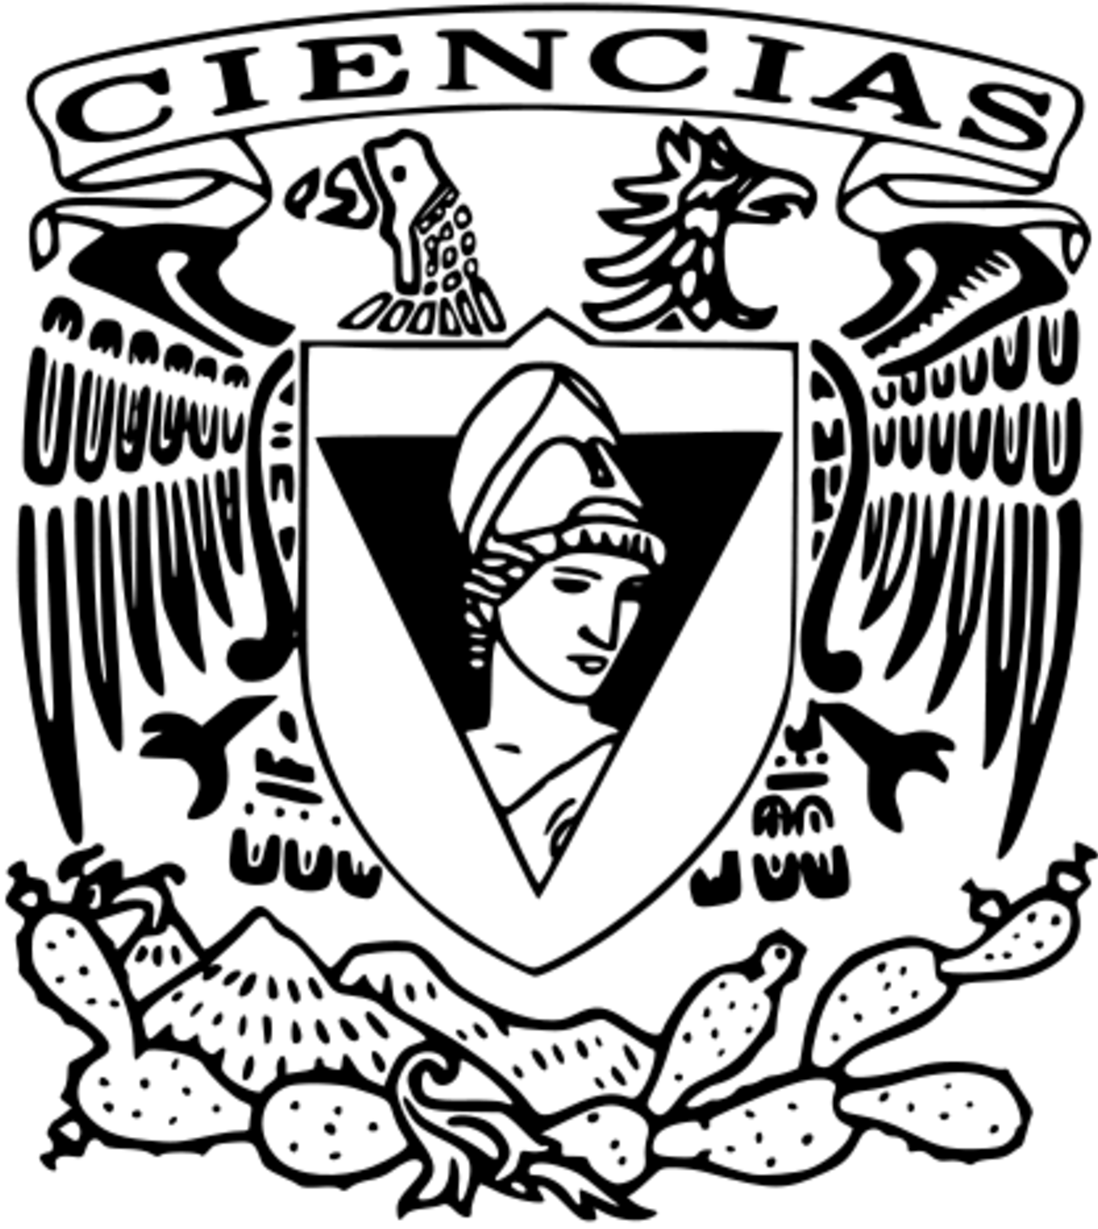
\includegraphics[height=3.4cm]{Logo_FC.png}
    	\end{center}
    \end{minipage}
\end{center}

\rule{17cm}{0.1mm}

%%%%%%%%%%%%%%%%%%%%%%%%%%%%
% FIN DE ENCABEZADO
%%%%%%%%%%%%%%%%%%%%%%%%%%%%

\begin{inciso}{Cono}
- Considera el cono que tiene como directriz la curva en coordenadas polares \( r = 2(1 - \cos \theta) \) con \( \theta \in [0, 2\pi] \) en el plano \( xy \) y vértice el punto \( V = (0, 0, 1) \).

\begin{problema}{Da la ecuación paramétrica del cono.}
-
\begin{multicols}{2}
    
Para empezar el problema, identificamos cuál es la directriz y cuál es el vértice: 
\begin{itemize}
    \item La directriz es la curva en coordenadas polares $r=2(1-\cos \theta)$ en el plano $xy \text{ con } z=0$
    \item El vértice del cono es $V=(0,0,1)$ 
\end{itemize}

Podemos graficar tanto la curva como el vértice en geogebra, dándonos cuenta que es un punto sobre un cardioide aplastado sobre el plano $xy$. 

\begin{figure}[H]
    \centering
    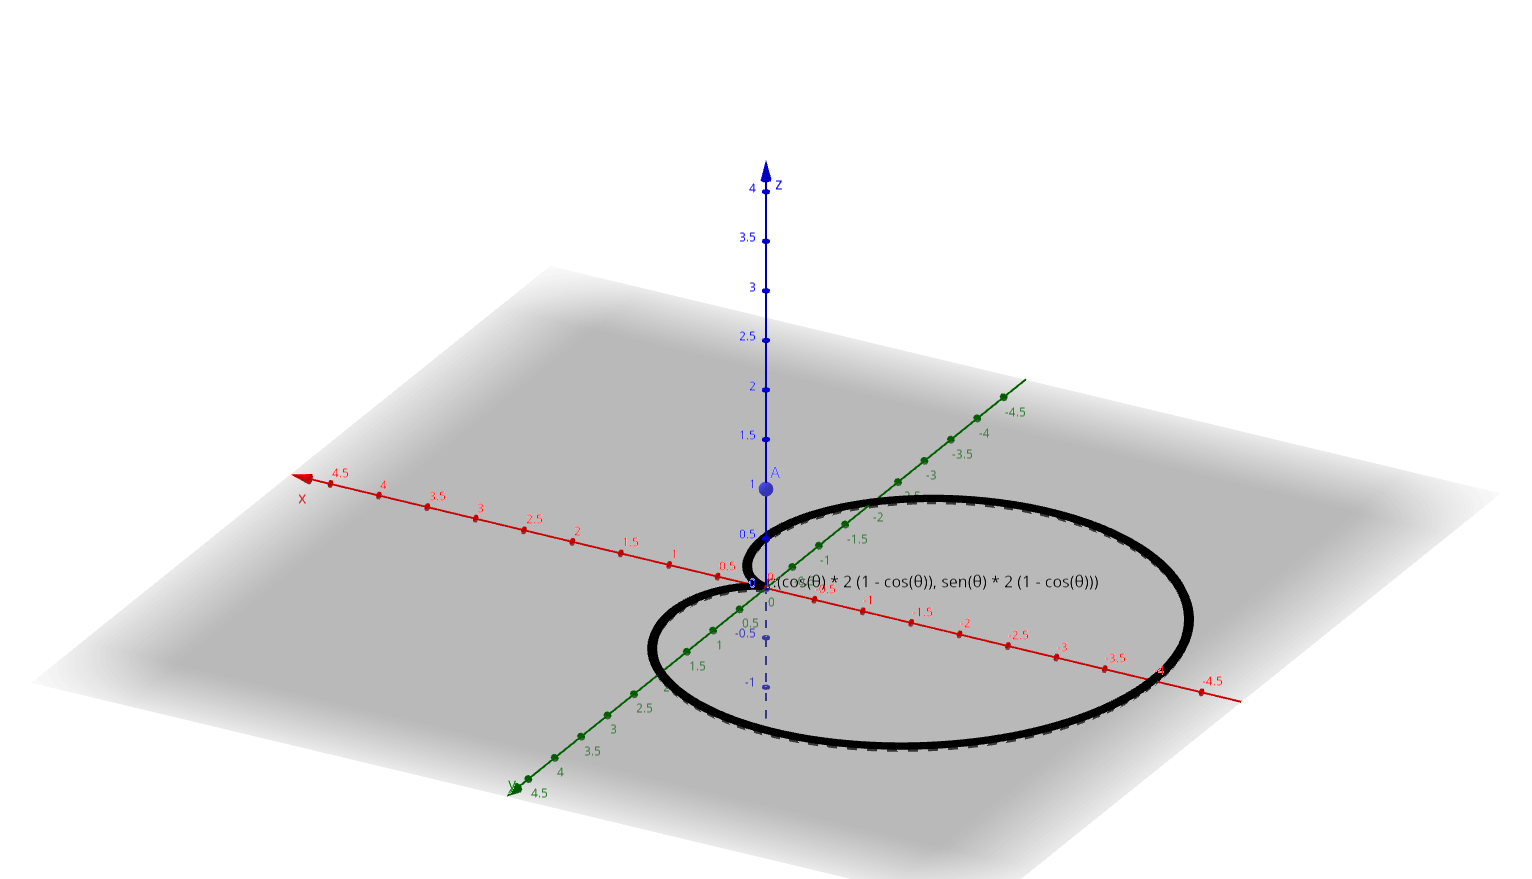
\includegraphics[height=4.3cm]{curva.png}
\end{figure}
Seguidamente de ésto, la idea ahora es parametrizar la directriz en coordenadas cartesianas: Usando $x=r \cos \theta$ y $y=r \sin \theta$, sustituimos $r=2(1-\cos \theta)$
\begin{equation*}  
    \begin{split}
        x(\theta)&=2(1-\cos \theta)\cos \theta, \\
        y(\theta)&=2(1- \cos \theta)\sin \theta, \\
        z(\theta)&=0. 
    \end{split}
\end{equation*}
    
Ahora bien, tenemos que parametrizar las generatrices del cono, las cuales son rectas que unen el vértice $V$ con cada punto $ \alpha(\theta) = (x(\theta), y(\theta), 0) $ de la directriz. Para ello, introducimos un parámetro $ s \in \mathbb{R} $ que controla la posición a lo largo de la generatriz, comportándose de la siguiente manera:  
\begin{itemize}
    \item Cuando $s = 0$, se está en el vértice $V$.
    \item Cuando $s = 1$, se está en la directriz $(z = 0)$. 
    \item Para $s > 1$, se extiende más allá de la directriz.   
\end{itemize}
\end{multicols}

Acto seguido, podemos proceder a escribir las ecuaciones paramétricas, la posición de un punto en el cono se obtiene interpolando linealmente entre $V$ y $\alpha(\theta)$, es decir, usando la definición de cono parametrizada $\psi (t,s)= \alpha (t) + s(V-\alpha(t))$:

\begin{center}
    
    $
    \begin{cases}
        x( t, s) = 0 + s \cdot 2(1 - \cos t)\cos t = 2s(1 - \cos t)\cos t, \\
        y( t, s) = 0 + s \cdot 2(1 - \cos t)\sin t = 2s(1 - \cos t)\sin t, \\
        z( t, s) = 1 + s \cdot (-1) = 1 - s.
    \end{cases}
    $
    
\end{center}

Cabe recalcar que podemos sustituir "$\theta$" por "$t$" para no entrar en confusiones con la notación que se ocupa usualmente en parametrización. \\
Por último, sólamente queda especificar los dominios de los parámetros y presentar la ecaución ya desarrollada: 
\\\\
\boxed{
\begin{minipage}{0.25\textwidth} 
    \begin{equation*}  
        \begin{split}
            &\psi: [0, 2\pi) \times \mathbb{R} \rightarrow \mathbb{R}^3, \\
            &t \longmapsto [0, 2\pi), \\
            &s \longmapsto \mathbb{R}.
        \end{split}
    \end{equation*} 
    \end{minipage}% 
    \begin{minipage}{0.75\textwidth} 
        \begin{center}
            $ \psi (t,s)=
            \begin{cases}
                x( t , s) = 2s(1 - \cos t )\cos t , \\
                y( t , s) = 2s(1 - \cos t )\sin t , \\
                z( t , s) = 1 - s,
            \end{cases} \quad \text{con }  t  \in [0, 2\pi), \ s \in \mathbb{R}.
            $
        \end{center}
    \end{minipage}
}

\end{problema}



\begin{problema}{Da la ecuación cartesiana del cono.}
-    
\begin{multicols*}{2}
    
    Tomamos las ecuaciones paramétricas del primer problema: 
    
    \begin{center}
    $
    \begin{cases}
        x( t , s) = 2s(1 - \cos t )\cos t , \\
        y( t , s) = 2s(1 - \cos t )\sin t , \\
        z( t , s) = 1 - s,
    \end{cases}
    $
\end{center}

Lo primero que debemos de hacer es eliminar el parámetro "$s$", es decir, de $z=1-s$, despejamos $s$: 
\begin{equation*}
    s=1-z.
\end{equation*}
Ahora bien, sustituímos $s$ en $x$ y $y$: 
\begin{equation*}
    \begin{split}
        x &= 2(1 - z)(1 - \cos t )\cos t , \\ 
        y &= 2(1 - z)(1 - \cos t )\sin t .
    \end{split}
\end{equation*}
Luego de ésto, tenemos que expresar $\cos t \text{ y } \sin t$ en términos de $x$ y de $y$: 

Sea $ A = 2(1 - z)(1 - \cos t) $, entonces:  
\begin{equation*}
    x = A \cos t, \quad y = A \sin t. 
\end{equation*}
Por lo tanto:  
\begin{equation*}
    \cos t = \frac{x}{A}, \quad \sin t = \frac{y}{A}.
\end{equation*} 

Usando $ \cos^2 t + \sin^2 t = 1 $:  
\begin{equation*}
    \left(\frac{x}{A}\right)^2 + \left(\frac{y}{A}\right)^2 = 1 \implies x^2 + y^2 = A^2.
\end{equation*}   
   Pero $ A = 2(1 - z)(1 - \cos t) $, así que:  
   \begin{equation*}
    \sqrt{x^2 + y^2} = 2(1 - z)(1 - \cos t).
\end{equation*} 
Como antepenúltimo paso, eliminamos $t$, sabiendo lo siguiente: 

De $ x = A \cos t $, se tiene $ \cos t = \frac{x}{\sqrt{x^2 + y^2}} $.  
   Sustituyendo en la ecuación anterior:  
   
\begin{equation*}
       \sqrt{x^2 + y^2} = 2(1 - z)\left(1 - \frac{x}{\sqrt{x^2 + y^2}}\right).
\end{equation*}   
   Multiplicando ambos lados por \( \sqrt{x^2 + y^2} \):  
\begin{equation*}
       x^2 + y^2 = 2(1 - z)\left(\sqrt{x^2 + y^2} - x\right).
\end{equation*}   
De ésta manera, sólo queda simplificar la ecuación llevando todos los términos a un lado: 
\begin{equation*}
    x^2 + y^2 + 2x(1 - z) = 2(1 - z)\sqrt{x^2 + y^2}.
\end{equation*}
\end{multicols*}
Al final, la ecuación cartesiana del cono queda cómo: 
\begin{center}
    $\boxed{
        x^2 + y^2 + 2x(1 - z) = 2(1 - z)\sqrt{x^2 + y^2}
        }$
    \end{center}
\end{problema}

\begin{problema}{Realiza la gráfica del cono.}
    -    

    \begin{figure}[H]
        \centering
        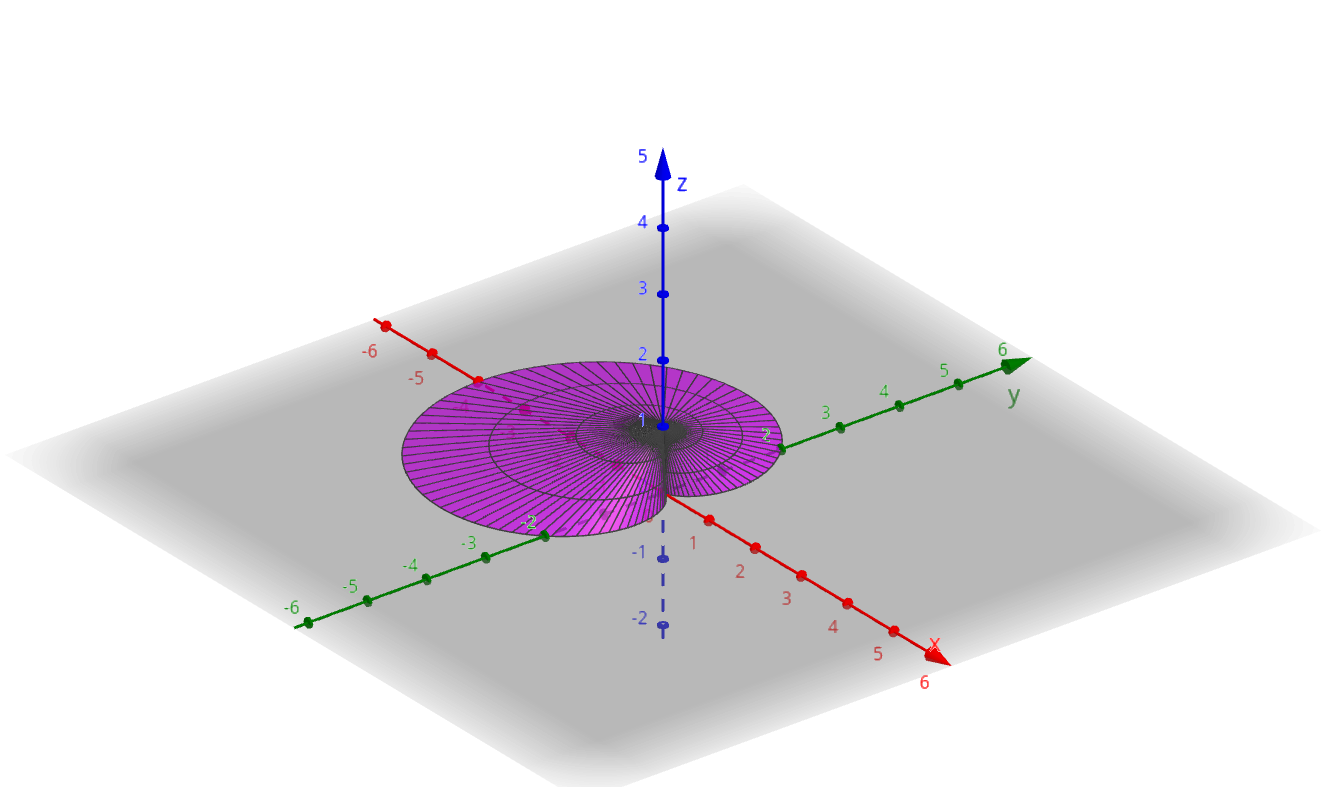
\includegraphics[height=6cm]{Cardioide-Cono.png}
    \end{figure}

\end{problema}

\end{inciso}

\begin{inciso} {Cilindro}
- Considera el cilindro cuya directriz es la hipérbola \( x^2 - y^2 = 1 \) y el vector de dirección es \( v = (1, 2, 1) \).

\begin{problema}{Da la ecuación paramétrica del cilindro.}
- 

Para construir la ecuación paramétrica, tomamos como punto generador cualquier punto de la hipérbola \(x^2 - y^2 = 1\) (por ejemplo, en el plano \(z=0\)) y le sumamos todos los vectores paralelos a \(v=(1,2,1)\).

Una forma natural de parametrizar la hipérbola es usando funciones hiperbólicas. Así, podemos escribir:
\[
x_0=\cosh u,\quad y_0=\sinh u,\quad z_0=0,\quad u\in\mathbb{R}.
\]
Entonces, un punto cualquiera del cilindro es:
\[
(x,y,z)=(\cosh u,\sinh u,0)+t\,(1,2,1),\quad t\in\mathbb{R}.
\]
Esto se traduce en el sistema:
\[
\begin{cases}
x=\cosh u + t,\\[1mm]
y=\sinh u + 2t,\\[1mm]
z=t.
\end{cases}
\]

Por último, sólamente queda especificarlos dominios de los parámetros y presentar la ecuación ya desarrollada: 
\\\\
\boxed{
\begin{minipage}{0.25\textwidth} 
    \begin{equation*}  
        \begin{split}
            &\psi: \mathbb{R} \times \mathbb{R} \rightarrow \mathbb{R}^3, \\
            &u \longmapsto \mathbb{R}, \\
            &t \longmapsto \mathbb{R}.
        \end{split}
    \end{equation*} 
    \end{minipage}% 
    \begin{minipage}{0.7\textwidth} 
        \begin{center}
            $\psi (u,t)=
            \begin{cases}
                x(u,t)=\cosh u + t,\\
                y(u,t)=\sinh u + 2t,\\
                z(t)=t,
            \end{cases} \quad \text{con }  u  \in \mathbb{R}, \ t \in \mathbb{R}.
            $
        \end{center}
    \end{minipage}
}

\end{problema}

\begin{problema}{Da la ecuación cartesiana del cilindro.}
- 

Para obtener la ecuación cartesiana del cilindro partimos de la parametrización del mismo. Una forma de parametrizarlo es:

\[
\begin{cases}
x=\cosh u+t,\\[1mm]
y=\sinh u+2t,\\[1mm]
z=t,
\end{cases}\quad u,t\in\mathbb{R}.
\]

Observamos que, al fijar \(t=z\), se puede escribir:

\[
x-z=\cosh u,\quad y-2z=\sinh u.
\]

Recordando la identidad hiperbólica
\[
\cosh^2 u - \sinh^2 u = 1,
\]
se concluye que para cualquier punto \((x,y,z)\) del cilindro se cumple:

\[
(x-z)^2 - (y-2z)^2 = 1.
\]

Al final, la ecuación cartesiana del cilindro queda cómo: 

\begin{center}
    $\boxed{
        (x-z)^2 - (y-2z)^2 = 1.
        }$
    \end{center}

\end{problema}

\begin{problema}{Realiza la gráfica del cilindro con el método visto en la sección 7.2 de las notas.}
- 

\begin{figure}[H]
    \centering
    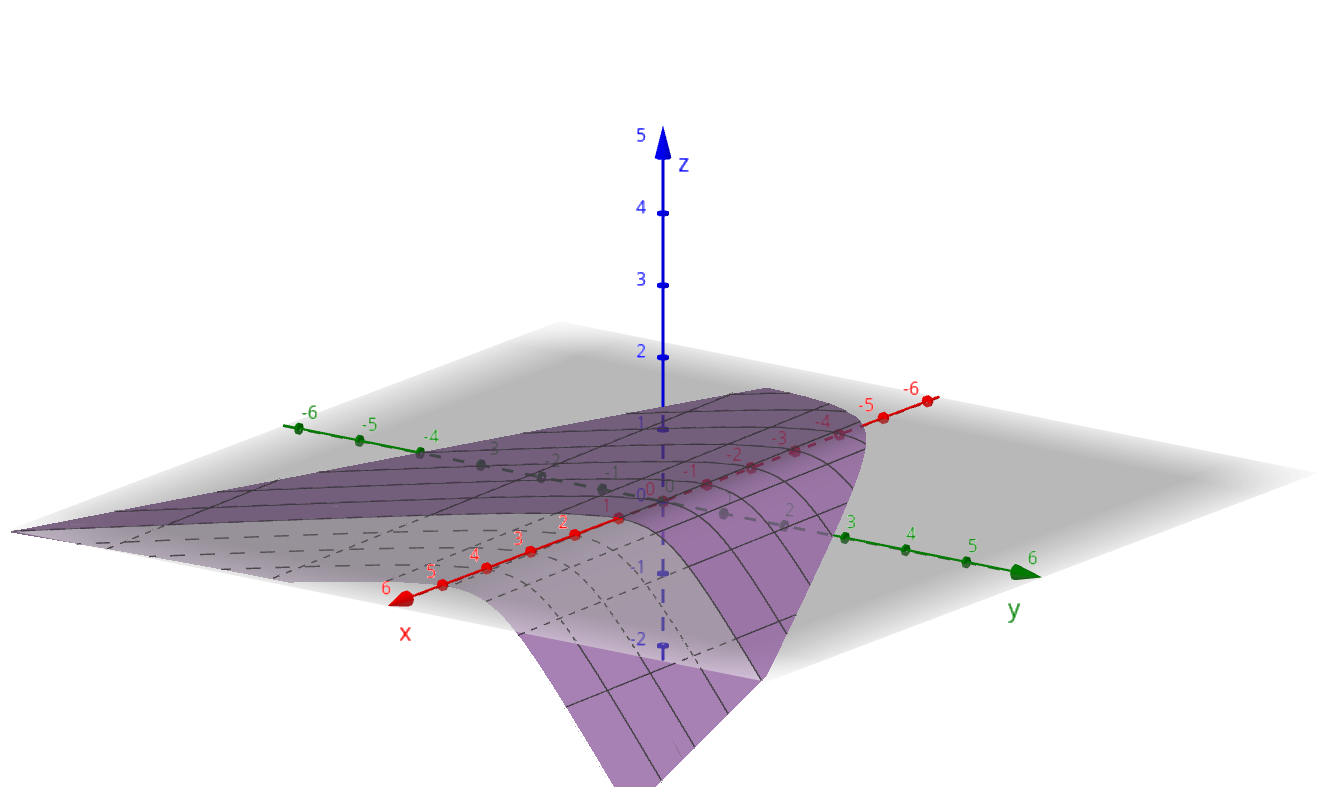
\includegraphics[height=6cm]{Cilindro-hipérbola.png}
\end{figure}

\end{problema}

\end{inciso}

\end{document}


    